\section{Agda Mechanization}\label{sec:mechanization}
Thus far, we have presented a system for pattern matching with typed holes, and we have discussed the reasoning and motivation for all of its aspects. Hopefully, the reader should find our system fairly intuitive, and should be reasonably convinced of its correctness. Indeed, we have provided various metatheoretical and semantic theorems which indicate that all of our judgements behave as expected, and that they enforce the constraints we desire.

However, even with such theorems stated and proved on-paper, we must consider that humans have quite a propensity for error. (After all, much of our work here focuses on analyses which seek to prevent common human errors!) Indeed, pattern matching with holes in both expressions and patterns can be very intricate, requiring reasoning about a three-valued logic of must, must not, and indeterminate judgments. Likewise, the proofs of our theorems involve large amounts of casework, considering many combinations of expressions, patterns, and constraints. Anecdotally, our initial work required nearly 150 pages of tediously typed out proofs. Thus, while on-paper proofs \emph{supposedly} show that our system is correct, it is highly unlikely that such voluminous work is entirely error-free.

To address this, and to provide a stronger guarantee of our system's correctness, we then must utilize something much more reliable than human intuition. Namely, we turn to the Agda proof-assistant \cite{norell:thesis}, providing a computer-checked mechanization of nearly all theorems stated here. Our mechanization is available for viewing at \href{https://github.com/hazelgrove/patterns-agda}{https://github.com/hazelgrove/patterns-agda}, and it is well-commented with documentation explaining the contents of each file. The only results we do not mechanize are those related to the $\cincon{\Xi}$ procedure discussed in \autoref{sec:decidability}. As previously mentioned, such proofs involve algorithms which use finite sets sets in a non-structurally recursive way, making them cumbersome to implement in Agda.

Throughout the rest of this section, we present an in depth discussion of our mechanization. In \autoref{sec:dependent-types}, we review the general background for dependently type theorem provers. Next, in \autoref{sec:mech-details}, we discuss how we encode our judgements, giving particular attentions to choices regarding binders, contexts, and other aspects that are often glossed over on paper. Finally, in \autoref{sec:errors}, we reflect on the benefit of our mechanization, enumerating the various subtle errors it revealed. 

\subsection{Theorem Proving with Dependent Types}\label{sec:dependent-types}
To begin, we review the required background on the Agda proof-assistant, discussing how its type system enables users to mechanically verify mathematical propositions. All of the material here is standard and should be familiar to the academic programming language researcher.

Briefly, Agda and other dependently-typed proof assistants function based on the following key observation: a type $T$ may be regarded as representing a proposition "$T$ is inhabited", and constructing a term $\ctyp{t}{T}$ correspondingly provides a proof of this proposition. If  our type system is sufficiently rich, we also have the converse: for any proposition $P$, we may construct a type $T_P$ such that "$T_P$ is inhabited" is logically equivalent to $P$, and the terms of $T_P$ are exactly the proofs of $P$. With such a type system, there is a one-to-one correspondence between propositions and types and between proofs and terms, commonly known as the \emph{Curry-Howard Correspondence} \cite{howard1980formulae}. 

Considering Agda in particular, it is a typed functional programming language based on a variant of Martin-L\"of type theory \cite{DBLP:books/daglib/0000395} known as the Unified Theory of Dependent Types \cite{DBLP:books/daglib/0078470, norell:thesis}. With dependent types, the division between types and values becomes blurry - types may be parameterized by arbitrary values, and types may be given as arguments and results of functions. Such a formulation is quite powerful, allowing Agda's type system to correspond with a variant of intuitionistic logic. 

Let us show a small taste of the details of this correspondence. For a simple example, take binary product types $A \times B$. As terms of $A \times B$ are of the form $\hpair{a}{b}$ where $\ctyp{a}{A}$ and $\ctyp{b}{B}$, the terms of $A \times B$ consist exactly of a proof of $A$ and a proof of $B$. Thus, $A \times B$ corresponds to the logical "and" of propositions $A \times B$. Indeed, \autoref{fig:product-and} shows that the type checking rules for $A \times B$ syntactically mirror the intuitionistic natural deduction rules for $A \land B$.

% !TeX root = thesis.tex
\begin{figure}[ht]

\begin{mathpar}
\Infer{\AndIntro}{ 
	\Gamma \vdash A \\ \Gamma \vdash B 
}{
	\Gamma \vdash A \land B
}

\Infer{\AndElimL}{
	\Gamma \vdash A \land B
}{
	\Gamma \vdash A
}

\Infer{\AndElimR}{
	\Gamma \vdash A \land B
}{
	\Gamma \vdash B
}

\Infer{\TAPair}{
	\Gamma \vdash a : A\\ \Gamma \vdash b : B
}{
	\Gamma \vdash (a, b) : A \times B
}

\Infer{\TAFst}{
	\Gamma \vdash p : A \times B
}{
	\Gamma \vdash \hfst{p} : A
}

\Infer{\TAFst}{
	\Gamma \vdash p : A \times B
}{
	\Gamma \vdash \hsnd{p} : B
}
\end{mathpar}
	
\caption{Correspondence between $A \times B$ and $A \land B$}
\label{fig:product-and}
\end{figure}


Analogously, binary sums $A + B$ correspond to the logical "or" of propositions $A \lor B$. For a more interesting case, consider propositions of the form $\forall x. B$, stating that for any $x$, the proposition $B$ holds, where $B$ may depend on $x$. In our correspondence, we can consider $B$ to be a type parameterized by a value $x$, say $x : A$ for some other type $A$. That is, $B$ is a \emph{dependent type}. To prove $\forall x..~ B$, we then must be able to produce a proof $f(a) : [a / x]B$ for any $a : A$. That is, we should have a function $f$ which takes inputs $a : A$ and produces outputs $f(a) : [a / x]B$. We refer to $f$ as a \emph{dependent function}, noting that its return type may depend on the particular value of its input. Formally, we write $f : \Pi_{x : A} B$. \autoref{fig:function-forall} shows a syntactic correspondence between type checking rules for dependent functions and natural deduction rules for universal quantification. 

% !TeX root = thesis.tex
\begin{figure}[ht]
	
	\begin{mathpar}
		\Infer{\UniversalIntro}{ 
			\Gamma \vdash B \\ \text{($x$ not free in $\Gamma$)}
		}{
			\Gamma \vdash \forall x. B
		}
		
		\Infer{\UniversalElim}{
			\Gamma \vdash \forall x. B
		}{
			\Gamma \vdash [a / x]B
		}
		
		\Infer{\TALam}{
			\Gamma , x : A \vdash b : B
		}{
			\Gamma \vdash \lambda x : A. b : \Pi_{x : A} B
		}
		
		\Infer{\TAAp}{
			\Gamma \vdash f : \Pi_{x : A} B \\ \Gamma \vdash a : A
		}{
			\Gamma \vdash f(a) : [a / x] B
		}
	\end{mathpar}
	
	\caption{Correspondence between $\Pi_{x : A} B$ and $\forall x. B$}
	\label{fig:function-forall}
\end{figure}


With the general idea of this correspondence now clear, let us present another feature of Agda we use pervasively in our development: \emph{inductive type families}. Briefly, an inductive type $T$ is specified by a finite list of functions with return type $T$, called \emph{constructors}, and the terms of $T$ consist of any syntactic form built up freely by repeated application of these constructors. In particular, the constructors themselves may inductively take arguments from $T$.

For example, recall the Peano construction of the natural numbers, where a natural number is either $0$ or inductively the successor of another natural number $suc(n)$. In Agda, we can represent this as an inductive type \li{Nat} as defined in \autoref{fig:naturals}. Here, there are two constructors: \li{zero} which takes no arguments, and \li{suc} which inductively takes a single argument of type $Nat$. The terms of \li{Nat} are then of the form \li{zero},\; \li{suc zero},\; \li{suc (suc zero)}, and so forth. Formally, the constructors yield the introduction rules shown in \autoref{fig:naturals}, and while not enumerated, appropriate elimination rules are also added, allowing functions to be defined by handling the case of each different constructor.

% !TeX root = thesis.tex
\begin{figure}[h]
\begin{subfigure}{.45\textwidth}
	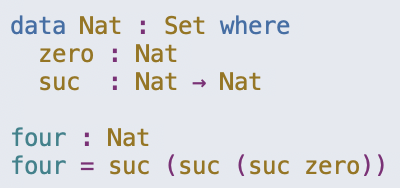
\includegraphics[scale=0.75,valign=t]{imgs/naturals.png}%
	\caption{Inductive Type Definition}
\end{subfigure}
\begin{subfigure}{.45\textwidth}
	\begin{mathpar}
		\Infer{\Zero}{
		}{
			\Gamma \vdash zero : Nat
		}\\
		\Infer{\Suc}{
			\Gamma \vdash n : Nat
		}{
			\Gamma \vdash suc~n : Nat
		}
	\end{mathpar}
	\caption{Introduction Rules}
\end{subfigure}
\caption{Natural numbers in Agda}
\label{fig:naturals}
\end{figure}

Inductive type families similarly define a family of types $T$, allowing $T$ to be parameterized by values or other types. With such inductive families, we can easily encode almost any mathematical judgement, letting $T$ represent the judgement and the constructors of $T$ represent the defining inference rules. For example, we can define a type $x < y$ parameterized by values $x~y : Nat$, specifying that $x$ is less than $y$. For any such $x, y$, one can prove $x < y$ either by the fact that $0 < n$, or by inductively using the fact that $m < n$ to get that $suc~m < suc~n$. Correspondingly, \autoref{fig:naturals-ordering} defines an inductive type family $\_{<}\_ : Nat \to Nat \to Set$ with two constructors. The relevant inference rules are also shown. Here, the syntax $\_{<}\_$ is a \emph{mixfix operator} where each $\_$ denotes an argument position and $x < y$ desugars to $\_{<}\_~x~y$. Additionally, arguments written with curly braces in the form $\{x : Nat\}$ are implicit and inferred by the compiler at call sites.

% !TeX root = thesis.tex
\begin{figure}[ht]
	\begin{subfigure}{.45\textwidth}
		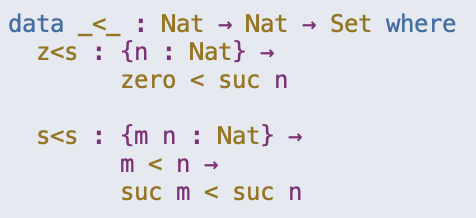
\includegraphics[scale=0.75,valign=t]{imgs/naturals-ordering.png}%
		\caption{Inductive Type Definition}
	\end{subfigure}
	\begin{subfigure}{.45\textwidth}
		\begin{mathpar}
			\Infer{\ZLessThanS}{
				\Gamma \vdash n : Nat
			}{
				\Gamma \vdash z{<}s : zero < suc~ n
			}\\
			\Infer{\SLessThanS}{
				\Gamma \vdash  m : Nat \\ \Gamma \vdash n : Nat \\ \Gamma \vdash p :  m < n
			}{
				\Gamma \vdash s{<}s~p : suc~m < suc~n
			}
		\end{mathpar}
		\caption{Introduction Rules}
	\end{subfigure}
	\caption{Ordering of natural numbers}
	\label{fig:naturals-ordering}
\end{figure}

\pagebreak

Considering the Curry-Howard correspondence, we can prove a theorem $\forall n \in \mathbb{N}, n < suc(n)$ by constructing a term of type $\Pi_{n : Nat}~n < suc~n$ as displayed in \autoref{fig:naturals-ordering-proof}. Note that Agda uses a more lightweight syntax for  $(n : Nat) \to  n < suc~n$ the dependent function type. The proof / function is defined by pattern matching, handling the case of each constructor analogously to an induction on derivations. Exhaustiveness checking guarantees that all cases are handled.

% !TeX root = thesis.tex
\begin{figure}[ht]
	\centering
	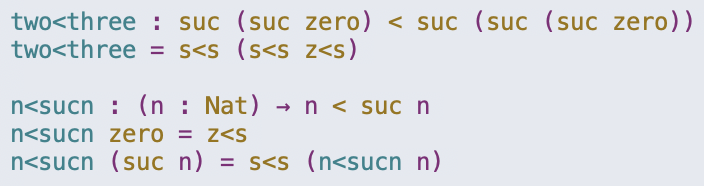
\includegraphics[scale=0.75,valign=t]{imgs/naturals-ordering-proof.png}%
	\caption{Example proofs using the ordering relation}
	\label{fig:naturals-ordering-proof}
\end{figure}

\subsection{Mechanization of Peanut}\label{sec:mech-details}
With the relevant background material discussed, we are now prepared to present the specifics of how we encode Peanut into Agda. Beginning with syntax, we can straightforwardly translate our grammars into inductive data types. We utilize mixfix operators and Agda's unicode support in order to closely mirror the on-paper notation. For example, \autoref{fig:agda-syntax} directly translates the syntax for constraints given in \autoref{fig:constraint} into an inductive data type.

% !TeX root = thesis.tex
\begin{figure}[ht]
	\centering
	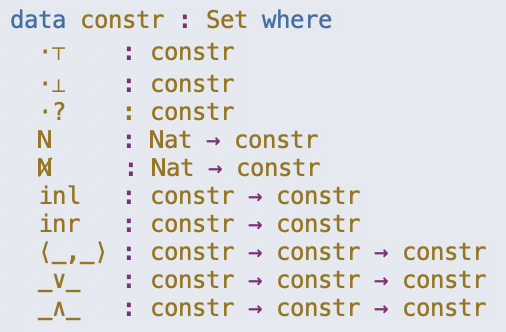
\includegraphics[scale=0.47,valign=t]{imgs/agda-syntax.png}%
	\caption{Constraint Language}
	\label{fig:agda-syntax}
\end{figure}

However, for usability reasons, our actual mechanization deviates slightly from the above definition of constraints. Explicitly, we instead define two separate constraint languages as shown in \autoref{fig:agda-constraints}. This formalizes the fact that we work with constraints in two distinct stages: first, the constraints directly emitted by lists of rules, then, for use in redundancy and exhaustiveness checking, the "fully-known" constraints which are in the image of the truify and falsify functions and their duals. The truify and falsify functions are then maps between these constraint languages. If we did not have such separation in our mechanization, we would continually have to pass around and reason about proofs that a constraint is fully know, and, morally, such changes are irrelevant.

% !TeX root = thesis.tex

\begin{figure}
	\centering
	% Capture tallest image in box 2
	\setbox2=\hbox{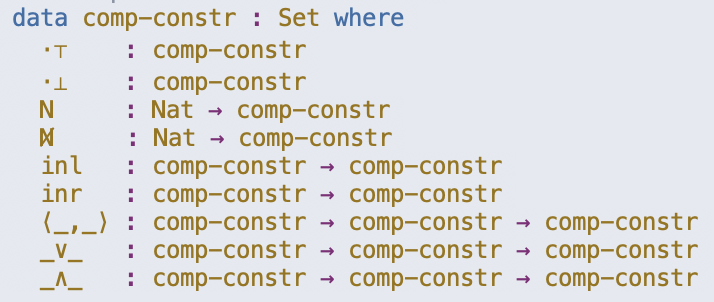
\includegraphics[scale=0.6]{imgs/agda-complete-constraints.png}}%
	\subcaptionbox{Incomplete Constraints}{
		\raisebox{\dimexpr\ht2-\height}{
			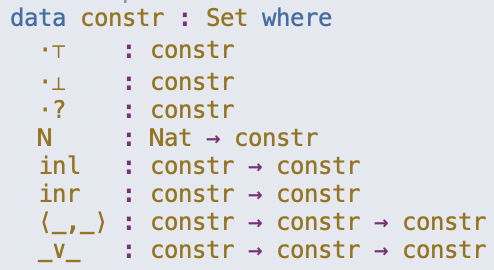
\includegraphics[scale=0.6,valign=t]{imgs/agda-constraints.png}
			\vphantom{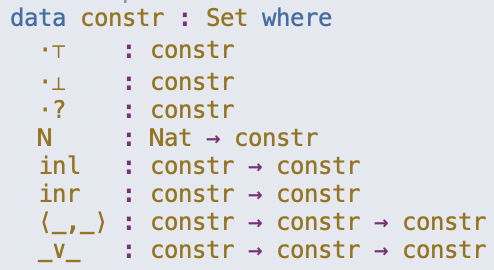
\includegraphics[scale=0.47,valign=t]{imgs/agda-constraints.png}}
		}
	}
	\hfil
	\subcaptionbox{Complete "Fully Known" Constraints}{
		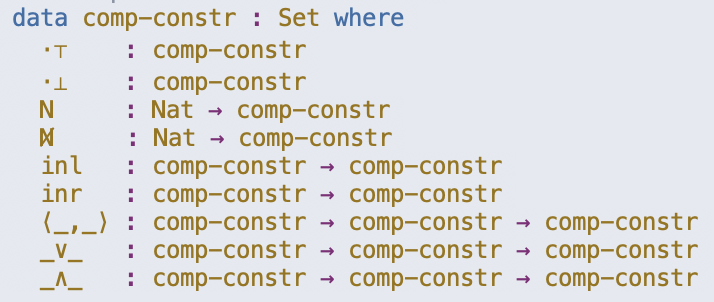
\includegraphics[scale=0.6,valign=t]{imgs/agda-complete-constraints.png}
	}
		\caption{Separated Constraint Languages}
	\label{fig:agda-constraints}
\end{figure}

The rest of the mechanization proceeds straightforwardly, with only a few other minor deviations from the paper which we will discuss shortly. Each judgement is encoded as an inductive type family, with its rules given by constructors there of. Mimicking the induction on derivations used for on-paper proofs about such judgements, all of our mechanized proofs proceed by pattern matching, handling the case of each constructor. 

However, it is worth noting that many details which are considered irrelevant on paper and frequently glossed must be explicitly handled in Agda. For example, consider \autoref{fig:agda-lambda}, which shows the Agda data type for our judgement $\hexptyp{\Gamma}{\Delta}{e}{\tau}$ and the constructor for the rule \TLam. For clarity, all other constructors of the data type are not displayed.

% !TeX root = thesis.tex
\begin{figure}[ht]
	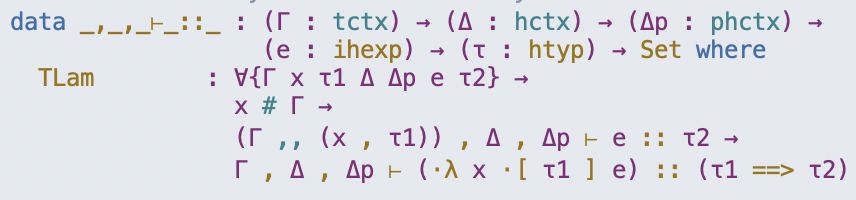
\includegraphics[scale=0.75,valign=t]{imgs/agda-lambda.png}
	\caption{Lambda Type Assignment}
	\label{fig:agda-lambda}
\end{figure}

The first two lines state that we are defining an inductive type family of the form $\Gamma, \Delta, \Delta_p \vdash e :: \tau$, where $\Gamma$ is a typing context, $\Delta$ is an expression hole context, $\Delta_p$ is a pattern hole context, $e$ is an expression, and $\tau$ is a type. Here, we see another small deviation from the paper, namely that our mechanization uses separate hole contexts for expression holes and pattern holes. Such a separation is irrelevant to the theory, but it is implemented with future developments in mind, e.g. if we later implement a fill-and-resume operation \`a la Hazelnut Live \cite{DBLP:journals/pacmpl/OmarVCH19}. 

In our mechanization, we implement contexts as metafunctions from variable names to optional contents, and for simplicity, we assume all variables are natural numbers. Correspondingly, the typing context $\Gamma$ above is a map $\text{Nat} \to \text{Maybe htyp}$. Whie not strictly required, in order to simplify working with such contexts, we also postulate function extensionality, which is known to be independent of Agda's axioms \cite{DBLP:conf/lics/AwodeyGS12}. We assume no other postulates in our development

Continuing, the next line defines a constructor \TLam. The type of this constructor begins with $\forall\{\Gamma~ \Delta~ \Delta_p~ e~ \tau\}$, specifying a number of implicit arguments which we instruct Agda to infer the type of. The following lines then correspond directly with the inference rules for \TLam, except notably, the inclusion of the premise $x \# \Gamma$. Such a premise specifies that $x$ does not occur  in $\Gamma$, which in terms of our implementation of contexts, specifies that $\Gamma~ x == \text{None}$. Why must we include this premise in our mechanization, while we do not on paper?

The core of the issue here is that on-paper presentations frequently ignore issues related to variable shadowing and conflict between free and bound variables. Instead, we implicitly assume that whenever required, $\alpha$-conversion can be performed as to rename any variables in the case of a conflict. However, for our mechanization, we must make an explicit of how to handle such conflicts. There are number of standard choices. For example, De Bruijn indices replace variables with a number indicating how many lambda abstraction there are between the variable use and where it bound, modifying these indices whenever required, and thereby removing any shadowing. Other approaches such as Abstract Binding Trees and Higher Order Abstract Syntax annotate the base syntax tree, explicitly tying binders to their scope and automatically performing rewriting when needed \cite{Harper2012}. However, in our experience, all of these approaches yield a pervasive overhead, quickly obfuscating the actual points of interest in our mechanization. As little of our theory depends on any specifics about binders, we choose to take a more lightweight approach known as Barendregt's convention \cite{DBLP:books/daglib/0067558, DBLP:conf/cade/UrbanBN07}.

Briefly, Barendregt's convention simply assumes that all binders and free variables are given globally unique names from the start. In our development, we then define a judgement specifying this, and wherever appropriate, insert such premises and disjointness assumptions between contexts. Returning to \autoref{fig:agda-lambda}, the premise $x \# \Gamma$ is an example of this, where we specify that lambda expressions are only well-typed if their binder is distinct from the free-variables recorded in the typing context. Again, we note that all these premises are benign, and can be discharged by $\alpha$-variation.

On a final note, our choice to follow Barendregt's convention did introduce a subtle issue in exactly one place in our mechanization: the rule \ITSuccMatch. In the case of a successful a pattern match $\hpatmatch{e}{p}{\theta}$, this rule applies the substitution $\theta$ to the corresponding branch expression for the rule. In our proof of \autoref{theorem:preservation}, following Barendreg'ts convention, we initially assume that the expression under consideration has globally unique binder names. Thus, applying the emitted subtitutions $\theta$ should ideally present no issues related to variable conflicts. However, in one specific case, namely, when the match succeeds due to the \MNotIntroPair rule, we may emit a substitution such as $[\hfst{e} / x,~ \hsnd{e} / y]$. When these substitutions are applied one by one, the latter substitution $[\hfst{e} / x]$ now replaces $x$ in a term that already has a copy of $e$, and thus has conflicting binders. Resultingly, the final expression may not be well-typed due to disjointness premises such as the one discussed in \autoref{fig:agda-lambda}.

% !TeX root = thesis.tex
\begin{figure}[ht]
	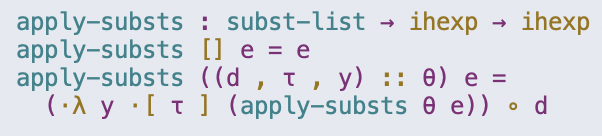
\includegraphics[scale=0.75,valign=t]{imgs/agda-substitutions.png}
	\caption{Expanding substitutions into lambdas}
	\label{fig:agda-substitutions}
\end{figure}

Luckily, we can resolve this issue with only a slight modification. When we apply $[\theta]e_r$ for our branch expression $e_r$, rather than actually performing the substitution, we wrap $e_r$ with appropriate lambda abstractions and applications as shown in \autoref{fig:agda-substitutions}. (The syntax $e_1 \circ e_2$ denotes function application in our mechanization). Effectively, this expansion defers the substitutions until later evaluation steps, and as a result, we can indeed re-apply Barendregt's convention between each substitution, resolving our issue. Unfortunately, however, as we only support half-annotated lambdas, this also requires $\theta$ to record typing information, which we ultimately achieve by adding a type annotation to the $\hpatmatch{e}{p}{\theta}$ judgement. Such annotations are benign, and are only required to handle this specific case.

\subsection{Issues Revealed by Mechanization}\label{sec:errors}
Finally, we reflect on the benefit that our mechanization provided, enumerating the various small issues that it revealed in the initial draft of our system. All of the issues here were revealed during mechanization, and were not discovered in the on-paper proofs of the same theorems.

As mechanization leaves no stone unturned, it is quite adept at revealing small subtle errors in our inference rules and judgements which are easy to overlook by a human. For example, consider the rules \IFst and \ISnd. Initially, these rules stated that for any expression $e$ with $\isIndet{e}$, we always have both $\isIndet{\hfst{e}}$ and $\isIndet{\hsnd{e}}$, a very intuitive statement. However, when mechanizing the fact that final expressions do not have applicable evaluation steps in \autoref{theorem:determinism}, it quickly became apparent that this conflicts with the stepping rules \ITFstPair and \ITSndPair, which allow taking projections of indeterminate pairs. Correspondingly, we updated \IFst and \ISnd to add the premise $e \neq \hpair{e_1}{e_2}$ as in their current version. From the mechanization of \autoref{theorem:determinism} alone, we also discovered that we had forgotten to allow evaluation steps under projections, requiring us to add the rules \ITFst and \ITSnd. Further, we discovered that the rules \ITApArg, \ITAp, and \ITPairR incorrectly specified various $\isVal{e}$ where there is now $\isFinal{e}$, again breaking progress. 

% !TeX root = thesis.tex
\begin{figure}[ht]
	
	\begin{mathpar}
		\Infer{\BadTRule}{
			p : \tau [\xi] \dashV \Gamma; \Delta_p \\
			\hexptyp{\Gamma_p \uplus \Gamma_p}{\Delta \uplus \Delta_p}{e}{\tau'}
		}{
			\chrultyp{\Gamma}{\Delta}{\hrulP{p}{e}}{\tau}{\xi}{\tau'}
		}\\
		\Infer{\GoodTRule}{
			\chpattyp{p}{\tau}{\xi}{\Gamma_p}{\Delta} \\
			\hexptyp{\Gamma \uplus \Gamma_p}{\Delta}{e}{\tau'}
		}{
			\chrultyp{\Gamma}{\Delta}{\hrulP{p}{e}}{\tau}{\xi}{\tau'}
		}
	\end{mathpar}
	
	\caption{Old and New Single Rule Typing}
	\label{fig:bad-ruletyp}
\end{figure}


Mechanizing the other half of type-safety, \autoref{theorem:preservation}, also proved useful. Initially, our judgement for pattern typing was syntactically written $p : \tau [\xi] \dashV \Gamma; \Delta$, rather than the current $\chpattyp{p}{\tau}{\xi}{\Gamma}{\Delta}$ defined in \autoref{fig:pat-rulestyp}. While the rules themselves were the same, the syntax here indicated that we conceptually considered both $\Gamma$ and $\Delta$ to be outputs, with $\Gamma$ recording variables bound in the pattern, and $\Delta$ recording hole names. Correspondingly, our rule typing judgement was initially stated as \BadTRule shown at the top of \autoref{fig:bad-ruletyp}, extending both $\Gamma$ and $\Delta$ to $\Gamma \uplus \Gamma_p$ and $\Delta \uplus \Delta_p$ when type checking the branch expression $e$. However, this is subtly incorrect, as it allows $e$ to include hole names which are also bound in $p$ but with conflicting typing information, and as our mechanization revealed, this results in the \ITSuccMatch rule stepping to an ill-typed expression. We corrected the rule correspondingly, as repeated in \GoodTRule in \autoref{fig:bad-ruletyp}.

For one small final error, mechanization also revealed the need for the $\possible{\xi}$ judgement discussed in \autoref{sec:constraints}. Without it, we would judge that an indeterminate expression $e$ indeterminately satisfies the $\bot$ constraint, despite the fact that no hole-filling would ever result in satisfaction.

We hope that our discussion here inspires the reader to take up the mechanization of their own work. Anecdotally, even beyond the errors identified, we found the mechanization extremely useful as we incrementally defined and extended our system. When changes are made, a robust mechanization makes it easy to determine which theorems must be updated, and if the theorems cannot be updated, it often obvious which parts of a definition are at fault. For one example, we extended our system with a unit type. While conceptually a very simple change, without mechanization, it would have required scanning through and updating all of our 150 pages of on-paper proofs. With the mechanization, however, the compiler immediately identified all proofs which were non-exhaustive, and with Agda's proof search capabilities, almost all the missing cases could be filled in automatically. 
